\begin{frame}{Jim's contributions}
\vspace{0.1 cm}

\Large
Good stuff.

\end{frame}

\begin{frame}{Case study: convergence of histogram libraries}
\vspace{0.5 cm}
The Scientific Python world lacked HEP-style histograms; it's one of the things we have to make ourselves.

\vspace{0.5 cm}
\uncover<2->{Also, it seems easy: just bin and count, right?}

\vspace{0.5 cm}
\uncover<3->{Physicists have created at least 20 histogram libraries in Python, most single-author.}

\vspace{0.5 cm}
\begin{uncoverenv}<3->
\begin{columns}
\scriptsize
\column{0.26\linewidth}
\begin{itemize}
\item PyROOT (2004--now)
\item PAIDA (2004--2007)
\item Plothon (2007--2008)
\item SVGFig (2008--2009)
\item YODA (2008--now)
\end{itemize}

\column{0.27\linewidth}
\begin{itemize}
\item DANSE (2009--2011)
\item rootpy (2011--2019)
\item SimpleHist (2011--2015)
\item pyhistogram (2015)
\item multihist (2015--now)
\end{itemize}

\column{0.28\linewidth}
\begin{itemize}
\item matplotlib-hep (2016)
\item QHist (2017--2019)
\item Physt (2016--now)
\item \mbox{Histogrammar (2016--now)\hspace{-0.2 cm}}
\item HistBook (2018--2019)
\end{itemize}

\column{0.32\linewidth}
\begin{itemize}
\item Coffea.hist (2019--2022)
\item boost-histogram (2019--now)
\item mplhep (2019--now)
\item histoprint (2020--now)
\item hist (2020--now)
\end{itemize}

\end{columns}
\end{uncoverenv}
\end{frame}

\begin{frame}{Histogram proliferation and convergence}
\vspace{0.25 cm}
\textcolor{darkblue}{Number of unique developers contributing to each library per month (in git).}

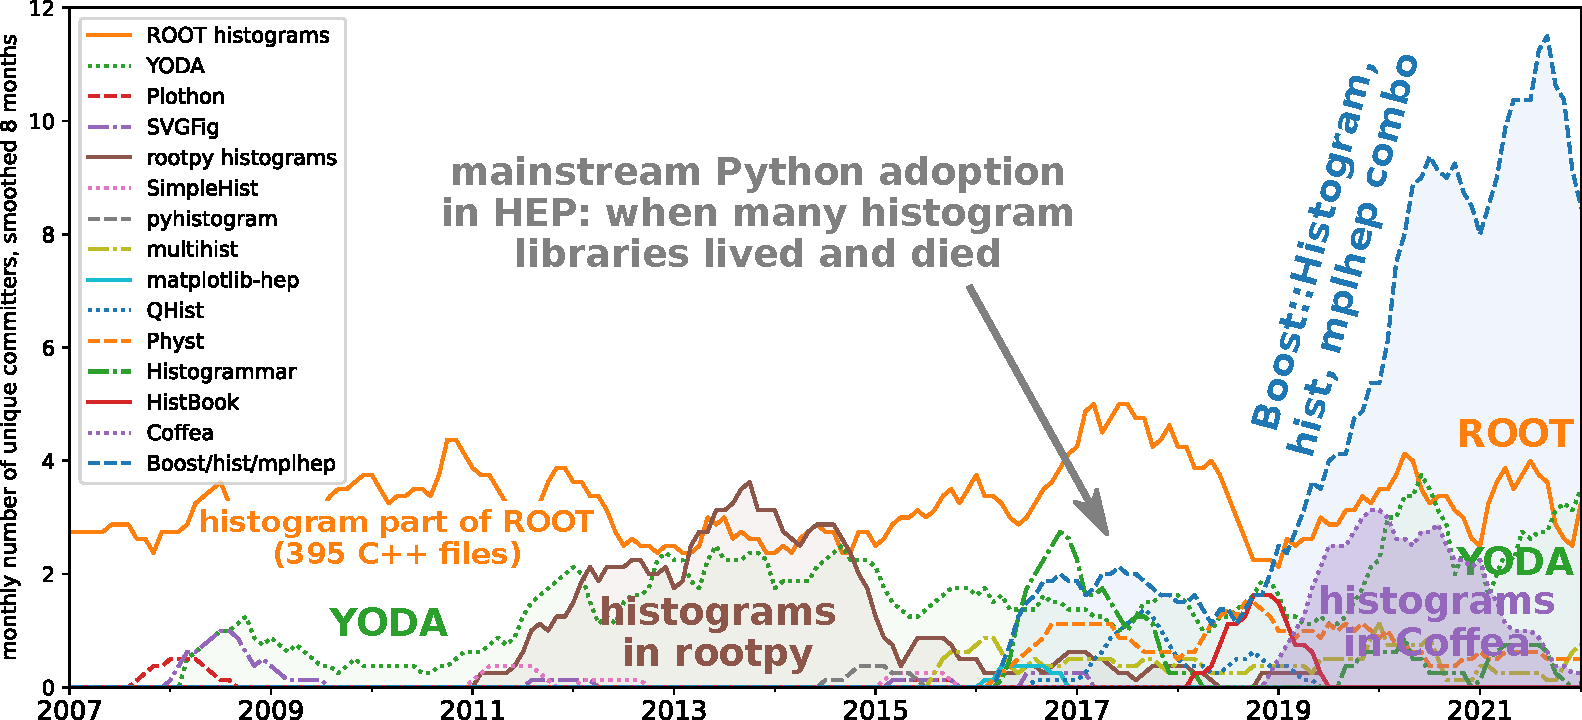
\includegraphics[width=\linewidth]{github-histogram-libraries.pdf}
\end{frame}

\begin{frame}[fragile]{Why combine Boost::Histogram, hist, mplhep?}
\vspace{0.5 cm}
\begin{columns}
\column{0.6\linewidth}
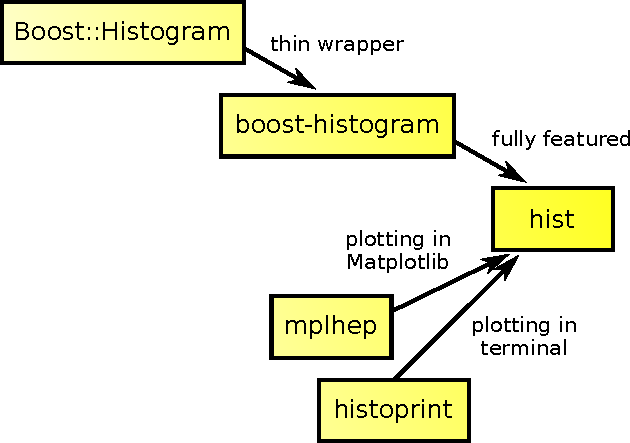
\includegraphics[width=\linewidth]{histogram-convergence.pdf}

\column{0.45\linewidth}
Originally, each of these was developed independently by a single author.

\vspace{0.75 cm}
\begin{uncoverenv}<2->
They each provide a piece of functionality users can get through

\begin{minted}{python}
import hist
\end{minted}
\end{uncoverenv}

\vspace{0.75 cm}
\uncover<3->{Now, 47 developers have contributed to these packages, and 20 contributed to more than one.}
\end{columns}
\end{frame}

\begin{frame}{Consistency maintained through agreed-upon protocols}
\vspace{0.5 cm}
\begin{columns}
\column{1.1\linewidth}
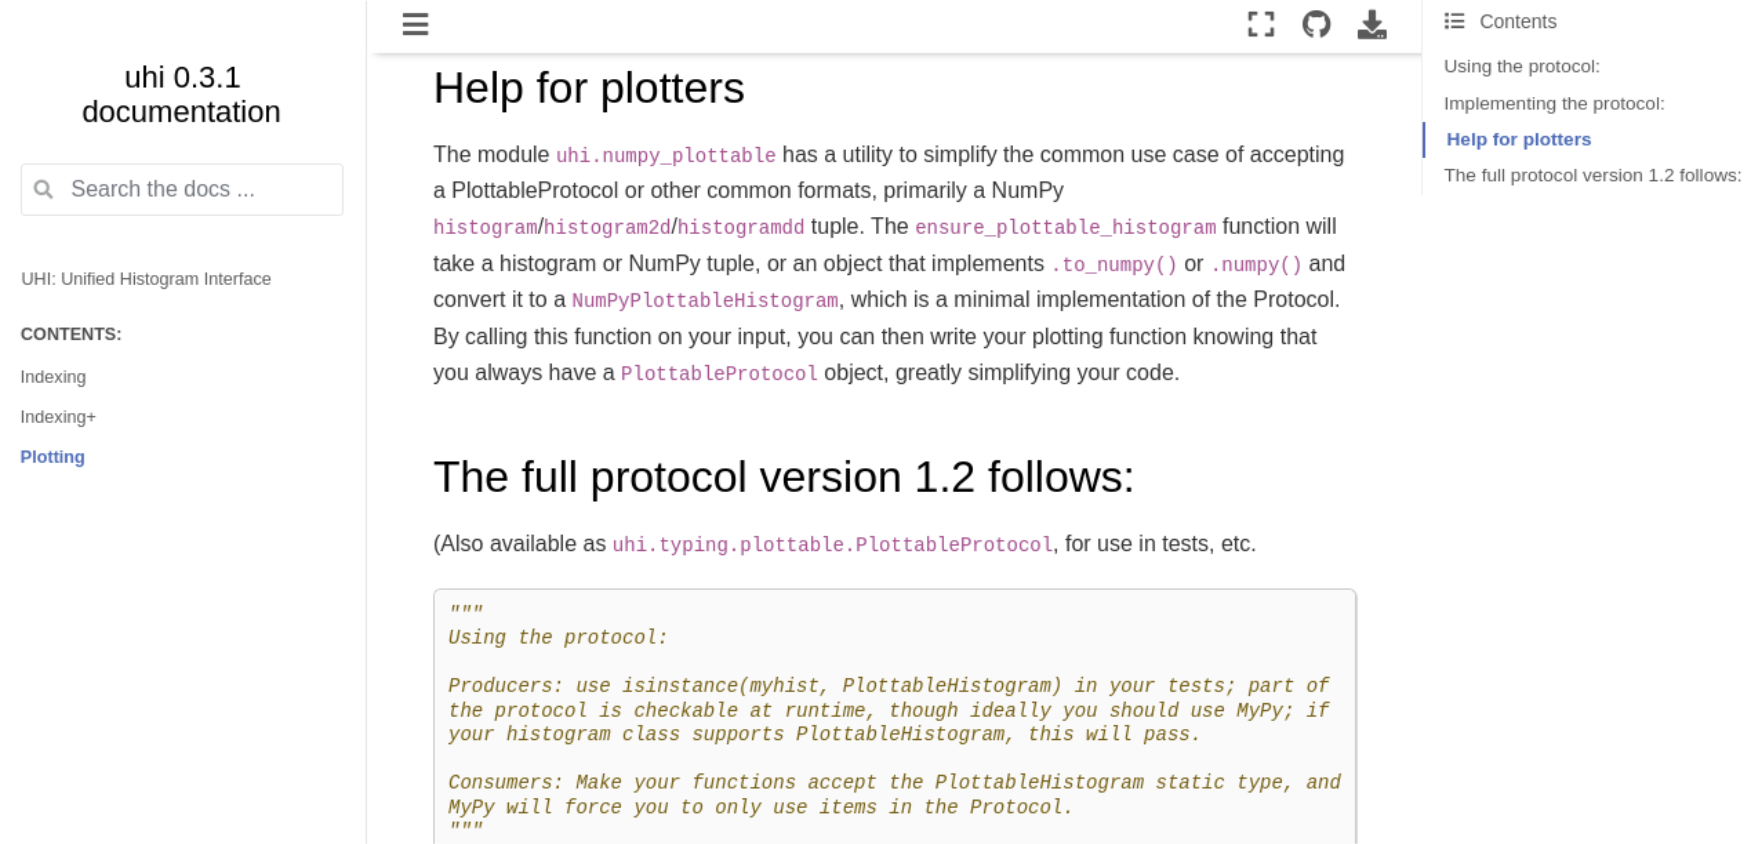
\includegraphics[width=\linewidth]{histogram-protocol-screenshot.png}
\end{columns}
\end{frame}

\begin{frame}{Another need: arrays of non-tabular data}
\large
\vspace{0.25 cm}

Almost all HEP data consists of variable-length lists and nested objects, which would be easiest to describe as JSON (though inefficient). To make use of NumPy-centric tools, we need a way of accessing such data in a NumPy-like way.

\begin{columns}
\column{1.05\linewidth}
\only<1>{
\includegraphics[width=\linewidth]{figures/pivarski-one-slide-summary-0.pdf}}\only<2>{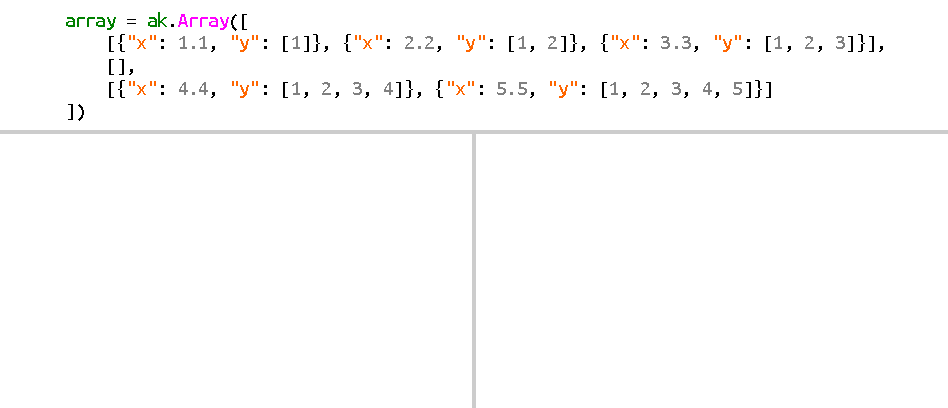
\includegraphics[width=\linewidth]{figures/pivarski-one-slide-summary-1.pdf}}\only<3>{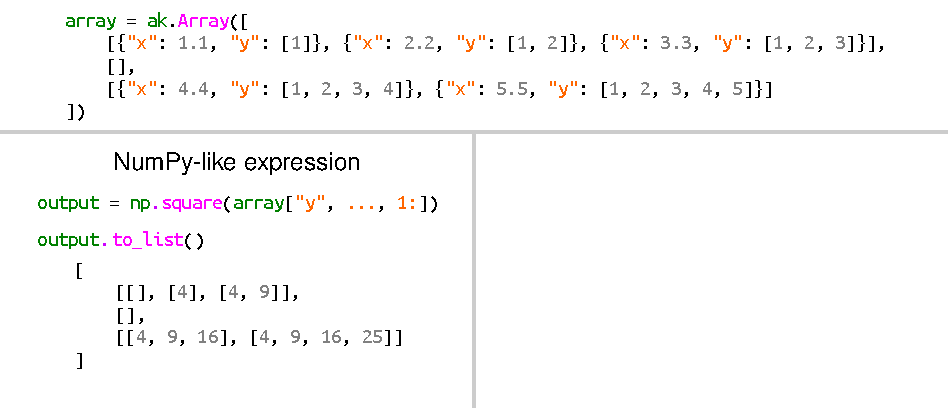
\includegraphics[width=\linewidth]{figures/pivarski-one-slide-summary-2.pdf}}\only<4>{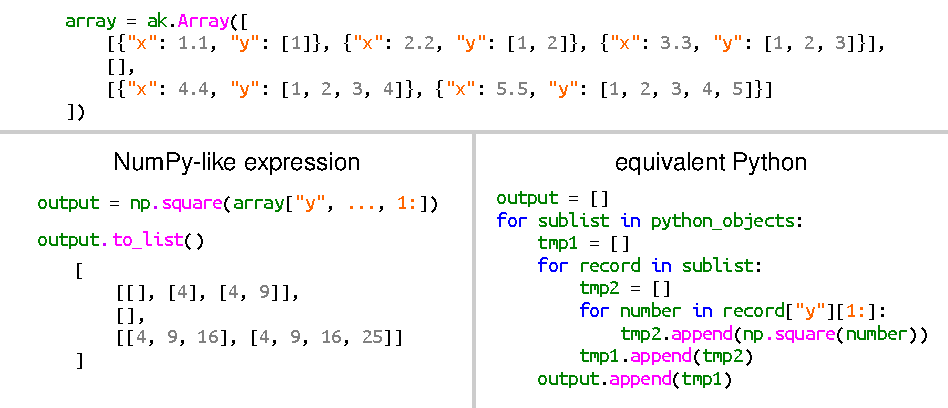
\includegraphics[width=\linewidth]{figures/pivarski-one-slide-summary-3.pdf}}
\end{columns}
\end{frame}
